\lecture{25 Feb.}

At the end of the last chapter, we characterize the behavior of codes in the asymptotic regime due to the fact that they are easier to compute and analyze. This chapter starts off by developing the essential tools in obtaining these concentration inequalities. Further, the Shannon's channel coding theorem on noisy channels is also introduced as an inspiration on how information is possible to be transmitted through erroneous channels.

Next, we delve into the theory and analysis of polar codes over noisy channels. Using tools such as the martingale theory, we see how the many observations mentioned from the last chapter are actually derived.

\section{Concentration Inequalities}
Given a collection of random variables, say $X_1$, $X_2$, $\ldots$, and $X_n$, that may or may not be independent or identically distributed, we would like to \textit{control} their joint distribution. A way to control their joint distribution is to bound their moments, an example would be to assume that they are independent and identically distributed (i.i.d.), then we know that
\begin{equation*}
    \frac{X_1+\cdots+X_n}{n} \approx \mathbb{E}[X_1].
\end{equation*}
The following theorem will be to characterize in what way does ``$\approx$'' hold.

\begin{theorem}[Hoeffding's Inequality]
    For i.i.d. R.V.s $X_1$, $\ldots$, and $X_n$, there exists a real number $c>0$ dependent on the distribution such that
    \begin{equation}
        \mathrm{Pr}\left\{\frac{X_1+\cdots+X_n}{n} - \mathbb{E}[X_1] \ge t\right\} \le \exp\left(-cnt^2\right).
    \end{equation}
\end{theorem}
The exact value to $c$ doesn't matter, and may vary from text to text. All that one has to know is that as long as $n\rightarrow\infty$, the bound approaches zero exponentially.

Let us consider a simple example on Bernoulli random variables and see that the Hoeffding's inequality indeed holds.
\begin{example}
    Consider i.i.d. $X_1$, $\ldots$, $X_n\sim\mathrm{Ber}(0.5)$ and $t>0$, we have
    \begin{align*}
        \mathrm{Pr}\left\{\frac{X_1+\cdots+X_n}{n} - \frac{1}{2} \ge t\right\} &= \mathrm{Pr}\left\{X_1+\cdots+X_n \ge n\left(t+1/2\right)\right\} \\
        &= \mathrm{Pr}\left\{\exp\left(s(X_1+\cdots+X_n)\right) \ge \exp\left(s\left(nt+n/2\right)\right)\right\}.
    \end{align*}
    This holds for all $s<0$, hence
    \begin{align*}
         \mathrm{Pr}\left\{\frac{X_1+\cdots+X_n}{n} - \frac{1}{2} \ge t\right\} &\le \inf_{s>0} \frac{\mathbb{E}\left[\exp\left(s(X_1+\cdots+X_n)\right)\right]}{\exp\left(s(nt+n/2)\right)} \\
        &= \inf_{s>0} \frac{\left[\frac{1}{2}(1+\ee^s)\right]^n}{\exp\left(s(nt+n/2)\right)}\;\;\;\;\;(\text{consider the MGF}) \\
        &\eqdef \exp(-cn),
    \end{align*}
    where
    \begin{equation*}
        c = \frac{1}{2}(2t+1)\ln\left(\frac{1+2t}{1-2t}\right) + \ln\left(1-2t\right) \gtrsim 2t^2 > 0.
    \end{equation*}
    Thus, it is shown. The right hand side to the first inequality written above is known as the Chernoff bound.
\end{example}


\begin{remark}
    There are two ways to generalize the Hoeffding's inequality:
    \begin{enumerate}
        \item find the best $c$.
        \item use non-i.i.d. random variables.
    \end{enumerate}
    
    Amazingly, if the random variables ${X_i}'s$ are correlated, or even not identically distributed, we can still obtain similar results! But the details are more technical.

    Consider the example on Bernoulli R.V.s above, replacements are required in calculating the expectation $\mathbb{E}\left[\exp(s(X_1+\cdots+X_n))\right]$. We need a different way to bound this expectation.

    This introduces us to the theory of \textit{sub-Gaussian random variables}. A random variable is called sub-Gaussian if $\mathbb{E}[\ee^{tX}] < \ee^{ct^2}$ for some constant $c$. This definition is motivated by the bounding of the tail probability: for $t>0$,
    \begin{equation}
        \mathrm{Pr}\{X\ge t\} = \mathrm{Pr}\left\{\exp(sX)\ge\exp(st)\right\}  \le \mathbb{E}[\exp(sX)] \ee^{-st} = \ee^{cs^2-st} \stackrel{s=\frac{t}{2c}}{=} \ee^{-\frac{t^2}{4c}}.
    \end{equation}
    All bounded random variables are sub-Gaussian. For a weaker decaying tail, one may use the \textit{sub-gamma random variables} to bound the tail probability.

    Another nice property of sub-Gaussians is that their sum concentrates the mean, hence we have that their average having a smaller and smaller variance. The same thing sadly does not apply for sub-Gammas.
\end{remark}

Besides the Chernoff bound and Hoeffding's inequality, the Chebyshev inequality and Markov inequality are also commonly used bounds. It is interesting to note that Chebyshev is actually the teacher of Markov and some may regard all the inequalities above as just special cases of Markov's inequality.




\section{Shannon's Noisy-Channel Coding Theorem}
A very well written paper which forms the onset of the information theory is C. E. Shannon's 1948 paper ``A Mathematical Theory of Communication'' \cite{Shannon}, in which the famous results such as source-channel separation, source coding, and channel coding are given.

\subsection{Channels}
In the first chapter, we have introduced terms such as capacity and rate, which are properties of a channel. So what exactly are channels? We shall illustrate them with examples.

The first three discrete channels shown below are, in order from left to right, \textit{binary erasure channel} (\textit{BEC}), \textit{binary symmetric channel} (\textit{BSC}), and Z-channel. The probability $p$ in BEC is termed the erasure probability; the probability $p$ in BSC is termed the cross-over probability.
\begin{figure}[H]
    \centering
    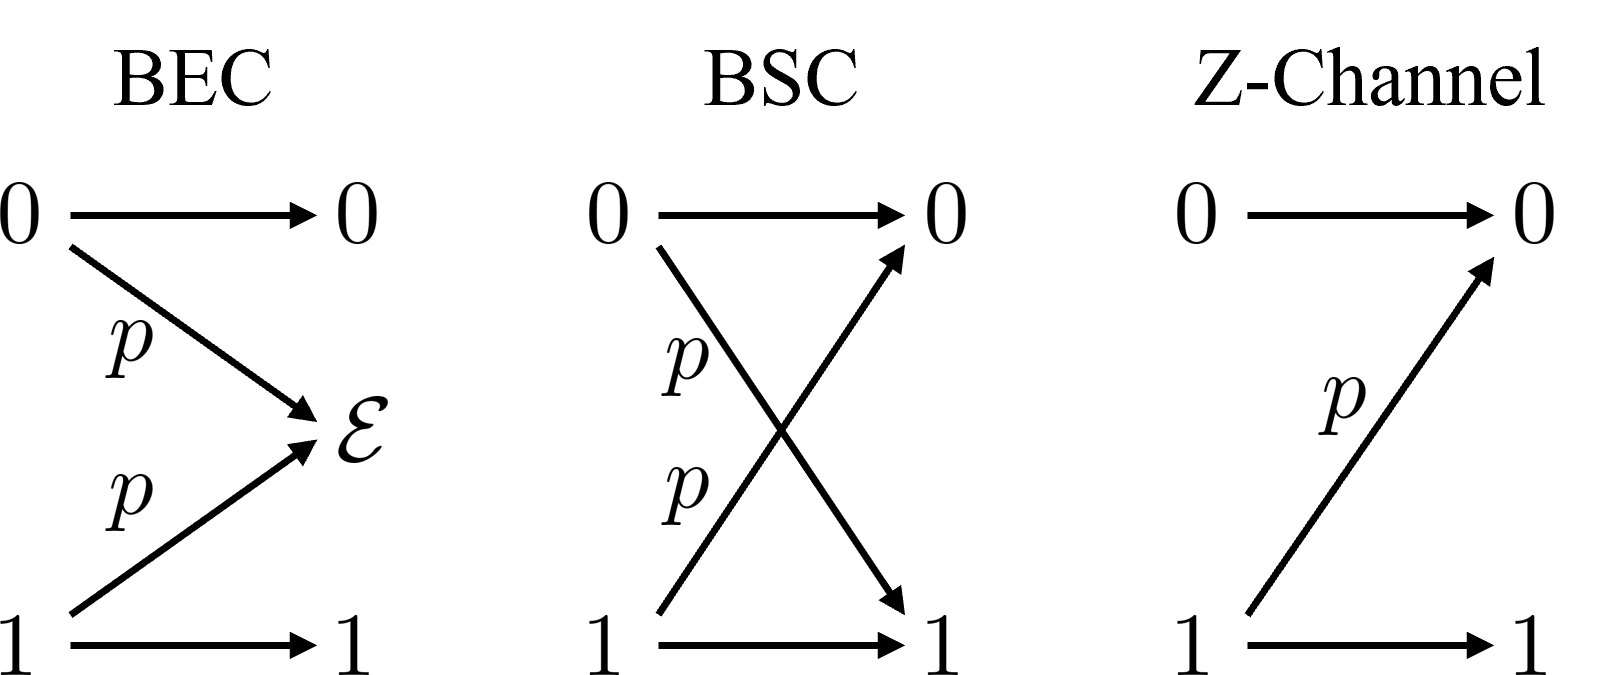
\includegraphics[width=0.5\linewidth]{figures/w2_discrete_channels.png}
    \caption{Some common channels: binary erasure channel, binary symmetric channel, Z channel.}
\end{figure}
Note that the Z-channel is a really bad channel. Though it seems to be a much simpler channel in comparison to BEC or BSC, it is bad since we cannot use linear code on it. The literature on linear code is so vast and widely used that if a channel cannot use linear code, the channel is deemed as a bad one.

Another example of a channel would be the continuous \textit{additive white Gaussian noise} (AWGN) channel. See the figure below, when an input bit is sent, a white (unbiased) Gaussian noise of variance $\sigma^2$ is added, resulting in a continuous spectrum of possible received signal.

\begin{figure}[H]
    \centering
    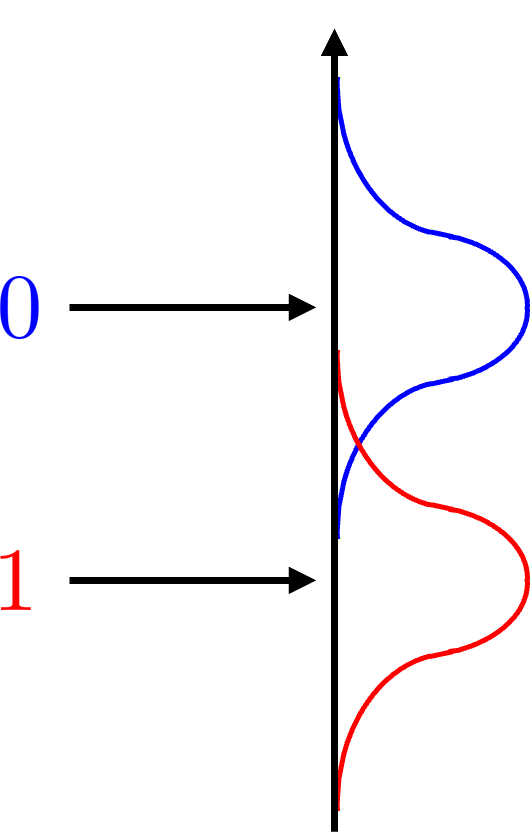
\includegraphics[width=0.15\linewidth]{figures/w2_AWGN.png}
    \caption{Additive white Gaussian noise channel.}
\end{figure}

In general, a discrete memoryless channel is characterized by the tuple $(\mathcal{X},\mathcal{Y},W)$, where the transition probability from $x\in\mathcal{X}$ to $y\in\mathcal{Y}$ is $W(y\vert x)$.

\subsection{Shannon's Noisy-Channel Coding Theorem}
Here we give a more hand-wavy description of Shannon's theory, relating the capacity, rate, allowed error of a channel with its possibility to transmit information.

\begin{theorem}[Noisy-Channel Coding Theorem]
    For a channel $W$, there exists a number $C(W)>0$, such that one can transmit $C(W)-\varepsilon$ bits per usage and guarantee the existence of a code with error probability arbitrarily small.
\end{theorem}

First off, this is a highly \textit{non-trivial} result! How is it even possible for one to transmit information in the face of noises and errors? 

Let us consider the following demonstration using BEC: select a subset $\mathcal{C}\subset\{0,1\}^n$ of \textit{codewords} for transmission. For example, in the case of $n=3$, the repetition code is $\mathcal{C}=\{000,111\}$, sending 000 if the message 0 is to be sent, sending 111 if the message 1 is to be sent. The repetition code has a code rate of $R=(\#\text{ of bits of information sent})/(\#\text{ of channel use}) = 1/3$. Can we do better? Yes, consider sending the message 1, 2, 3, and 4 with the codewords $\mathcal{C}=\{000,011,101,110\}$. This code has a code rate of $R=2/3$. And in the face of erasure, we can still determine the message most of the time: the decoder will be
\begin{align*}
    \mathrm{Dec}: 1\mathcal{E}0 &\mapsto 110 = \text{message 4} \\
    00\mathcal{E} &\mapsto 000 = \text{message 1} \\
    1\mathcal{EE} &\mapsto ?
\end{align*}
Notice that if two or more erasures occur, the above code will not have perfect reconstruction. But this is alright, since we can just try again and again to decrease the failure probability.

A characteristic of the above demonstration is that when we increase the code rate, the error probability also increases. In practical designs, we care more about the increasing code rate instead of reducing the error probability, after all, who knows the difference between $10^{-6}$ and $10^{-9}$?

Here we will give a more detailed example regarding the existence of a good coding scheme on BEC.
\begin{example}
    Consider transmission with the channel $\mathrm{BEC}(0.5)$. Suppose that $n$ is big, and we can pick a $\mathcal{C}\subset\{0,1\}^n$. How do we choose good codewords $\mathcal{C}$? A common strategy for theoretical analysis is by \textit{random coding}.

    First, let us consider picking random codewords $w^1$ and $w^2\in\{0,1\}^n$. Let us send $w^1$ over $W$ to obtain, for example
    \begin{equation*}
        W:w^1 = 0011011\ldots \mapsto 0\mathcal{E}110\mathcal{E}1\ldots=y,
    \end{equation*}
    a question will be to ask what is the error probability that $y$ is \textit{compatible} with $w^2$?

    The received $y$ will be compatible with $w^2$ if for all index $1$ to $n$, either $y_i=\mathcal{E}$, or that $w^2_i=y_i=w^1_i$, each happening with probability $\frac{1}{2}$ and $\frac{1}{2}\cdot\frac{1}{2}=\frac{1}{4}$. So the total probability of a single bit being compatible will be $\frac{3}{4}$. So as $n\rightarrow \infty$, $y$ is compatible with $w^2$ with a probability of $\left(\frac{3}{4}\right)^n\rightarrow0$, meaning the two are incompatible. Moreover, we know that $y$ is compatible with $w^1$ with a probability of $1-\left(\frac{3}{4}\right)^n\rightarrow1$, meaning we have a high probability of knowing $y$ is indeed $w^1$.

    
\end{example}
However good the success probability may be, the rate of the above scheme is $R=1/n\rightarrow 0$. Can we do any better?
\begin{example}
    Consider the same as above, but this time, we allow for a larger set of codewords: $\mathcal{C}=\{w^i\}_{i=1}^m$. By including $m$ codewords, we can ask the same question on the compatibility of $y$ with $w^2$, $w^3$, $\ldots$, and $w^m$, and obtain a \textit{lower} bound on the success probability being
    \begin{equation*}
        \mathrm{Pr}\{\text{success detecting $w^1$ from $y$}\} = 1-(m-1)\left(\frac{3}{4}\right)^n.
    \end{equation*}
    And by choosing $m\approx\frac{1}{100}\left(\frac{3}{4}\right)^n$, we have the success probability being approximately $99\%$ with a non-zero code rate of
    \begin{equation*}
        R = \frac{\# \text{ bits of information sent}}{\# \text{ channel use}} = \frac{\lg m}{n} = \frac{\lg\left(\frac{3}{4}\right)^n}{n} = 0.415,
    \end{equation*}
    where $\lg(\cdot)=\log_2(\cdot)$. This is a constant code rate scheme!
\end{example}
Note that for the $\mathrm{BEC}(0.5)$ channel, the theoretical limit is $R=0.5$, which is the capacity of the channel. We can certainly improve further, but what is the problem with our analysis above that made it not able to saturate the bound? The devils are in the details. The ``bad events'' have intersections, and the over-estimation of the error probability costs us some capacity. For example, the all erasure string $\mathcal{EE\ldots E}$ is compatible with all ${w^i}'s$. A more careful analysis should be able to achieve the bound.

\begin{remark}
    The above analysis utilizes random codes. But it is only good for theory, since the implementation of its encoder and decoder requires $\exp(\mathrm{O}(n))$ of calculations. In practice, we need \textit{low complexity codes}. As we will see later, polar codes has the complexity of $\mathrm{O}(n\lg n)$.
\end{remark}

As an end to this chapter on the noisy-channel theorem, let us also consider another example on BSC. What happens with BSC and random coding? Just on an intuitive level, one should be able to obserbe the following:
\begin{enumerate}
    \item The channel $\mathrm{BSC}(0.5)$ is a bad channel (though it is a really good random seed generator).
    \item Our analysis should use $\mathrm{BSC}\left(1/4\right)$ instead.
    \item The channel $\mathrm{BSC}\left(3/4\right) = \mathrm{BSC}\left(1/4\right)$ since one can simply flip the 0 and 1 after passing through the former to obtain the latter.
    \item Pick $w^i\in\{0,1\}^n$ randomly, send $w^1=00\ldots0$.
    \item Obtain $y$, compute compatibility with $w^1$ by \textit{Hamming distance}. One should obtain $d_\mathrm{H}(y,w^1)\approx \frac{n}{4}$.
    \item Compute the compatibility of $y$ with other codewords, for example, $d_\mathrm{H}(y,w^2) \approx \frac{n}{2}$.
    \item We can set the decoding algorithm to be: If $d_\mathrm{H}(y,w^i)<\frac{n}{3}$, then we determine it to be $w^i$.
    \item The above decoding scheme fails when: (w.p. = with probability)
    \begin{enumerate}[label=(\arabic*)]
        \item $d_\mathrm{H}(y,w^1) > \frac{n}{3}$, w.p. $\le\left(\frac{1}{4}\right)^{n/3}$ (define this error to be $\alpha$), or
        \item $d_\mathrm{H}(y,w^{i\neq1}) < \frac{n}{3}$, w.p. $\le \left(\frac{1}{2}\right)^{2n/3}$ (define this error to be $\beta$).
    \end{enumerate}
    \item We can further bound the above via Chernoff bound: for $i=1\sim n$, let $F_i=1$ if the $i$th bit of $w^1$ is flipped to obtain $y$, else it is 0, then
    \begin{equation*}
        \alpha = \mathrm{Pr}\left\{F_1+\cdots+F_n\ge\frac{n}{3}\right\} = \mathrm{Pr}\left\{\frac{F_1+\cdots+F_n}{n} - \frac{1}{4}\ge\frac{1}{12}\right\} \le \exp(-cn).
    \end{equation*}
    \item Similarly, for $i=1\sim n$, let $X_i=1$ if the $i$th bit of $w^{i\neq1}$ is the same as $y_i$, else it is 0, then
    \begin{equation*}
        \beta = \mathrm{Pr}\left\{X_1+\cdots+X_n\ge\frac{2n}{3}\right\} = \mathrm{Pr}\left\{\frac{X_1+\cdots+X_n}{n} - \frac{1}{2}\ge\frac{1}{6}\right\} \le \exp(-c'n).
    \end{equation*}
    \item The total error probability is hence upper bounded by $\exp(-cn) + (m-1)\exp(-c'n)$.
    \item Consider the number of codewords to be $m\approx \frac{1}{100} \ee^{c'n}$, the code rate will hence be a constant $R\approx c'\lg e$, with success probability in decoding to be $\approx 99\%$. To obtain the exact value to the channel capacity (maximum possible code rate), one needs to solve a min-max program. Finally, with hard work, one should obtain that the channel capacity to be $C(p)=1+p\lg(p)+(1-p)\lg(1-p) = 1-(\text{binary entropy function})$.
\end{enumerate}

\section{Polar Code over BEC}
Consider again the binary erasure channel with a ``magical decoder'' as shown in the figure below.
\begin{figure}[H]
    \centering
    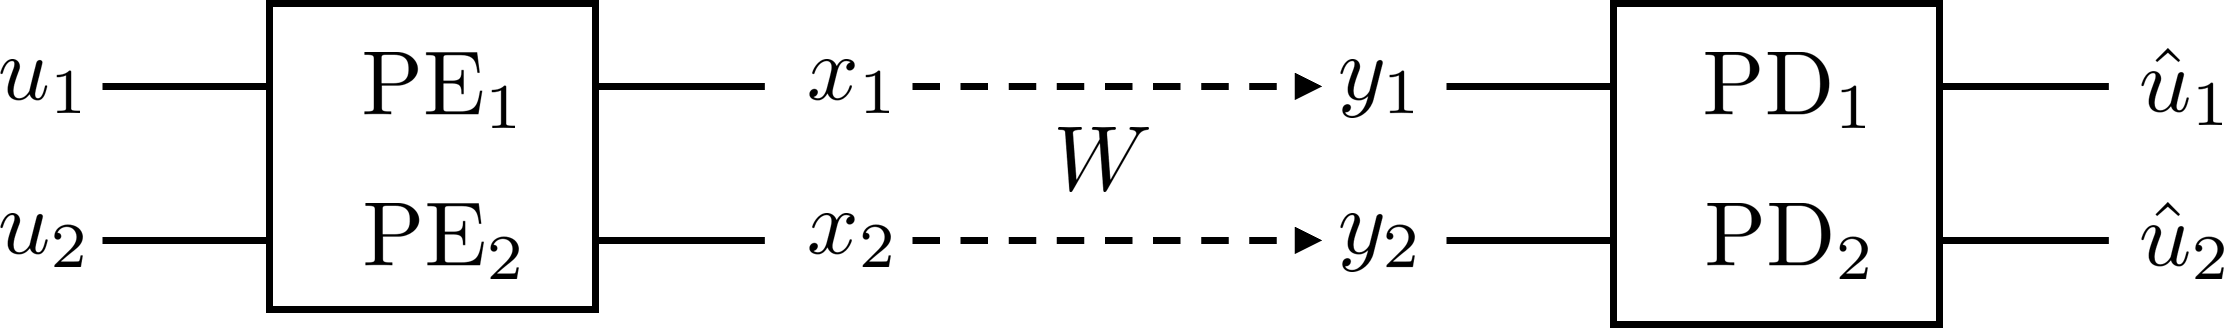
\includegraphics[width=0.6\linewidth]{figures/w2_split_channel.png}
    \caption{A single block for polar code encoding and decoding.}
\end{figure}
We have the polar encoders
\begin{equation}\begin{aligned}
    x_1\defeq \mathrm{PE}_1(u_1,u_2) &= u_1 \oplus u_2, \\
    x_2\defeq \mathrm{PE}_2(u_1,u_2) &= u_2.
\end{aligned}\end{equation}
The channel is
\begin{equation}
    W=\mathrm{BEC}(p),\; W(x)=\begin{cases}
        x &\text{w.p. } 1-p,\\
        \mathcal{E} &\text{w.p. } p.
    \end{cases}
\end{equation}
The polar decoders are
\begin{equation}\begin{aligned}
    \hat{u}_1\defeq \mathrm{PD}_1(y_1,y_2) &= \begin{cases}
        y_1 \oplus y_2 &\text{if $y_1\neq\mathcal{E}$ and $y_2\neq\mathcal{E}$}, \\
        \mathcal{E} &\text{otherwise;}
    \end{cases} \\
    \hat{u}_2\defeq \mathrm{PD}_2(y_1,y_2,u_1) &= \text{best guess of $u_2$}= \begin{cases}
        y_2 &\text{if $y_2\neq\mathcal{E}$,}\\
        y_1\oplus u_1 &\text{if $y_1\neq\mathcal{E}$ and $y_2=\mathcal{E}$,}\\
        \mathcal{E} &\text{otherwise.}
    \end{cases}
\end{aligned}\end{equation}
Note that the $u_1$ used in $\mathrm{PD}_2$ is \textit{the real one}, and not an estimate. These are the magical decoders used.

\subsection{Multi-Layered Polar Code}
We can combine it to form a two-layer polar code as below:
\begin{figure}[H]
    \centering
    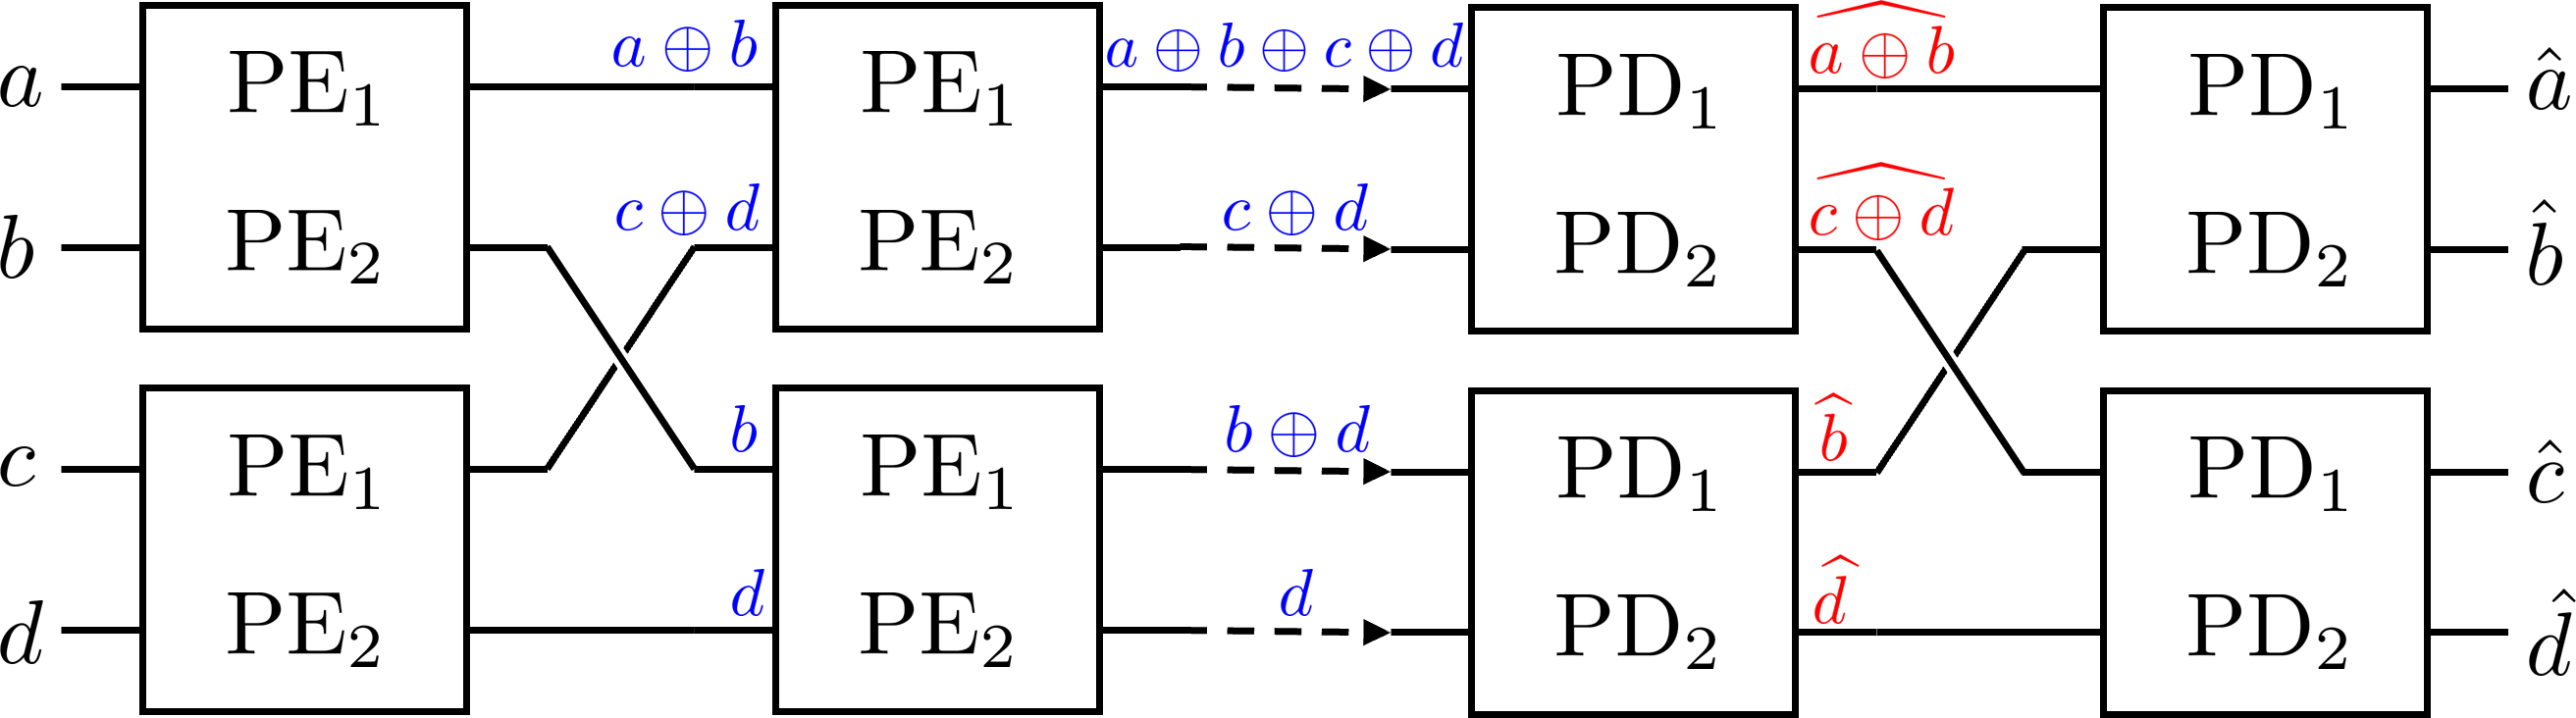
\includegraphics[width=0.7\linewidth]{figures/w2_polar_2layer.png}
    \caption{Two-layer polar code.}
\end{figure}
The variables with hats $\widehat{(\cdot)}$ once again represent estimates. On each transmission line, the variables being sent is also marked. We can further extend to a three-layer one, as shown in \autoref{fig:w2_polar_3layer}.
\begin{figure}[h]
    \centering
    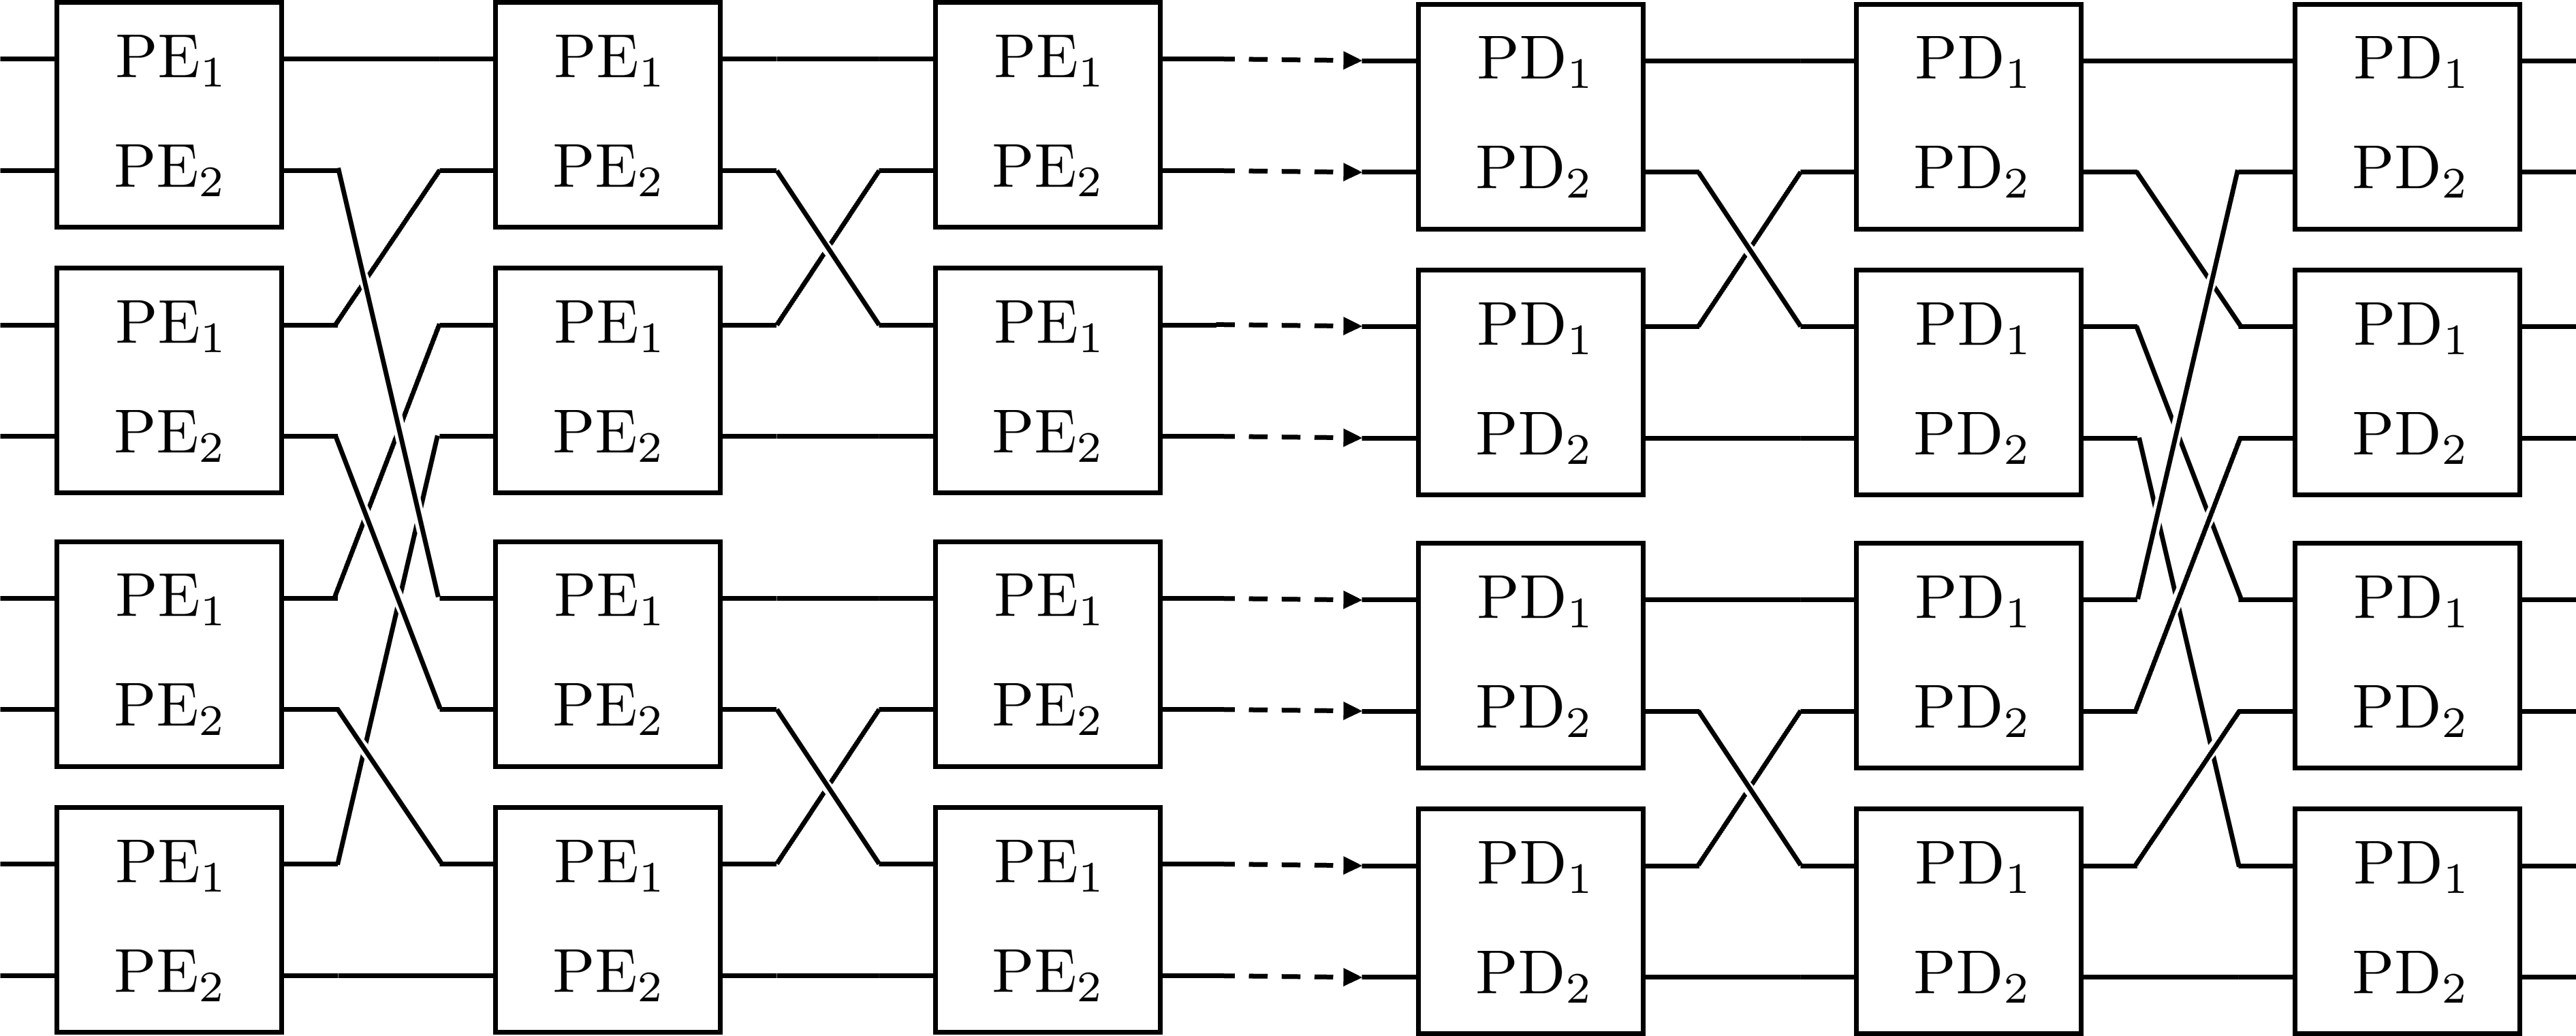
\includegraphics[width=0.8\linewidth]{figures/w2_polar_3layer.png}
    \caption{Three-layer polar code.}
    \label{fig:w2_polar_3layer}
\end{figure}
Amazingly, the structure of the encoder bears close resemblance to the \textit{butterfly diagram} used in the circuitry realization of the fast Fourier transform (FFT)! For $n$ bit inputs, the FFT algorithm has a computation complexity of $\mathrm{O}(n\lg n)$. Henceforth, the encoder structure of polar code has the operation complexity of $\mathrm{O}(n\lg n)$ as well. Random codes, on the other hand, though very useful for theoretical analysis, has a complexity of $\exp(O(n))$.

Finally, note that even though we draw the decoder also in the form of a butterfly diagram, it is not implemented so. Since $\mathrm{PD}_2$ requires the \textit{true value} to $u_1$ in calculating $\hat{u}_2$, the decoders are completed in an intertwined manner: The $\mathrm{PD}_1$'s are first calculated to obtain the required real values of $u_2$ for the $\mathrm{PD}_2$'s. As an exercise, one should check that for both the two-layer and three-layer polar code above, what is the order in which the $\mathrm{PD}_1$'s and $\mathrm{PD}_2$'s are performed? One can refer to the procedure shown in \autoref{fig:w3_polar_decoder} as a hint.

\subsection{Polar Code on BSC}
The same structure can be extended to $W=\mathrm{BSC}(p)$, the encoders can remain the same, however, the decoders need to be modified to a case-wise decision map. I.e., define the log-likelihood ratio function $\mathrm{LLR}(u\vert\theta) = \ln \left(\mathrm{Pr}\{u=0\vert\theta\} / \mathrm{Pr}\{u=1\vert\theta\}\right)$,
\begin{equation}\begin{aligned}
    \mathrm{PD}_1(y_1,y_2) &= \left[\phi\left(u_1\middle\vert\, y_1,y_2\right) \underset{1}{\overset{0}{\gtrless}} 0\right],\\
    \mathrm{PD}_2(y_1,y_2,u_1) &= \left[\phi\left(u_2\middle\vert\, y_1,y_2,u_1\right) \underset{1}{\overset{0}{\gtrless}} 0\right].
\end{aligned}\end{equation}
The value of $\phi$ needs to be determined case-wise. Even though it is more complicated than the BEC case, it still only requires finitely many steps, and hence the polar code works on BSC even in practical cases.

